% !TEX TS-program = pdflatex

\documentclass[unicode,11pt,notheorems,xcolor=table]{beamer}
\usepackage{fix-cm}
\usepackage[T2A]{fontenc}
\usepackage[utf8]{inputenc}
\usepackage[russian]{babel}
\usepackage{amsmath,amsfonts,amssymb,amsthm}
\usepackage{mathtools}
\usepackage{diagbox}

\usepackage{ulem}
\usepackage{tikz}
\usepackage{graphicx}
\usepackage{pgfplots}
\pgfplotsset{compat=1.16}

\usetikzlibrary{matrix,arrows,decorations.pathmorphing, arrows.meta,positioning}
\usetikzlibrary{positioning,calc}
\usetikzlibrary{patterns}
\usetikzlibrary{decorations.pathreplacing}

%Описание стиля презентации
\usetheme[sidebar=0]{kfmn} 
\setbeamercovered{transparent}

%\definecolor{cyan}{RGB}{240,217,1}
%\definecolor{vgugreen}{RGB}{143,188,103}
%\definecolor{vgured}{RGB}{234,38,40}
%\definecolor{vgublue}{RGB}{53,101,167}
\hypersetup{colorlinks,linkcolor=,urlcolor=blue}

\makeatletter
	\g@addto@macro{\endtabular}{\rowfont{}}% Clear row font
	\makeatother
	\newcommand{\rowfonttype}{}% Current row font
	\newcommand{\rowfont}[1]{% Set current row font
		\gdef\rowfonttype{#1}#1\ignorespaces%
	}
\makeatother

\newcommand{\myunit}{9mm}
\tikzset{
    node style sp/.style={draw,circle,minimum size=\myunit},
    node style ge/.style={circle,minimum size=\myunit},
    arrow style mul/.style={draw,sloped,midway,fill=white},
    arrow style plus/.style={midway,sloped,fill=white},
}

%[0, 6, 8, 8, 10, 5, 6, 10, 8, 10, 10], 

\pgfdeclareimage[height=8mm]{university-logo}{logo-iem.png}
\logo{\pgfuseimage{university-logo}}
%2[0, 11, 10, 8, 11, 5, 11, 11, 8, 11, 10, 11],

\titlepicture{
	\begin{tikzpicture}[y=1.4cm,overlay,rotate=8]
	\coordinate (O) at (-3cm,0.9cm);
	\filldraw[thick,draw= vgublue, fill=vgublue!20!white] (0,0) circle[radius=4.2cm];
	\clip (0,0) circle[radius=4.2cm];
	\draw (-1.5,1.5) node{
	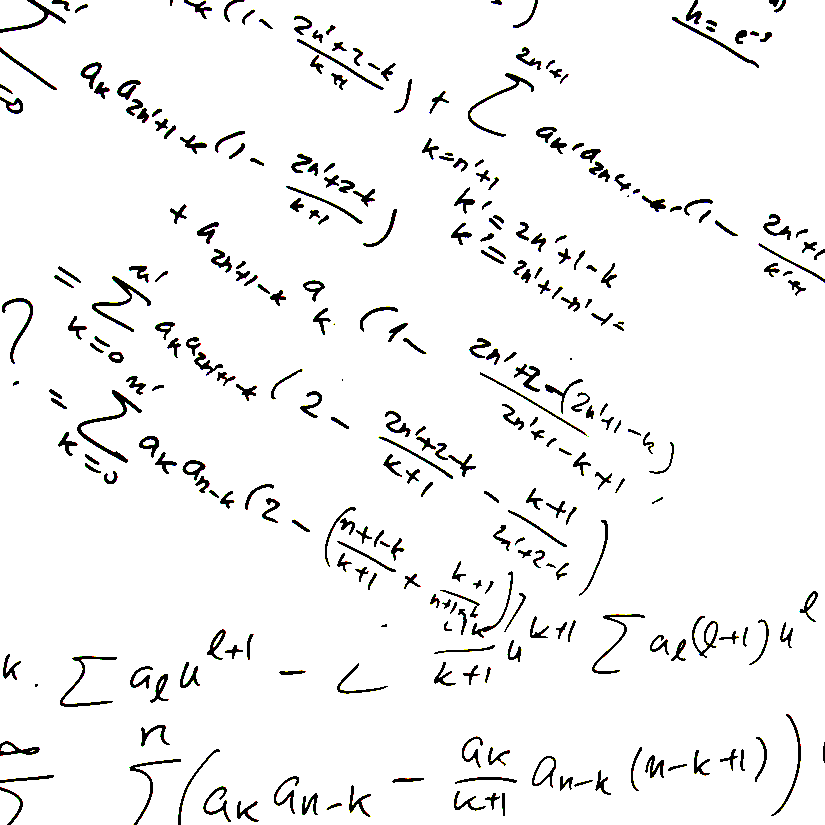
\includegraphics[width=8cm]{titlepic.png}
	};
\end{tikzpicture}
}

\usepackage[math]{iwona}

\newcommand{\hplus}{\mathbin{\hat+}}
\newcommand{\hdot}{\mathbin{\hat\cdot}}
% Описание теорем
\newtheorem{theorem}{Теорема}
\newtheorem{seq}{Следствие}
%%

\LECT % 

% Титульный лист теорем
\author[Д.\,В. Чупраков]{канд.\,физ.-матем.\,наук, доцент Д.\,В. Чупраков\\[6pt] usr10381@vyatsu.ru}

\institute[ВятГУ]{ФГБОУ ВО Вятский государственный университет}

\department{Факультет экономики и финансов}

\title[Лекция~18. Проверка гипотез -- 1]{
	Введение в экономико-математическое моделирование\\[12pt]
	Лекция~18. Проверка гипотез}
\date{9 декабря 2020~г.}


\setbeamercovered{invisible}

\setbeamercolor{math text}{fg=vgured!70!black}

\pgfmathdeclarefunction{gauss}{2}{%
  \pgfmathparse{1/(#2*sqrt(2*pi))*exp(-((x-#1)^2)/(2*#2^2))}%
}
\begin{document}


\maketitle

 \begin{frame}{Структура лекции}{}
 	\tableofcontents
 \end{frame}

\section{}

\begin{frame}{Статистическая гипотеза}{}

    \begin{block}{Определеине}
    \alert{Статистическая гипотеза}
    это предположение
    \begin{itemize}
        \item о виде распределения генеральной совокупности или 
        \item о величинах неизвестных параметров известного распределения генеральной совокупности,
    \end{itemize}
    которое может быть проверено на основании выборочных показателей.
    \end{block}

    По количеству предположений гипотезы делятся на:
    \begin{itemize}
        \item простые~--- это гипотезы, содержащие только одно предположение;
        \item сложные~--- гипотезы, состоящие из конечного или бесконечного числа простых гипотез.    
    \end{itemize}
\end{frame}
    % Проверка статистической гипотезы заключается в сопоставлении некоторых статистических показателей, вычисленных по данным выборки со значениями этих же показателей, определенных теоретически в предположении, что проверяемая гипотеза верна.



\begin{frame}{Mortal Combat}{}

\includegraphics[width=\textwidth]{vs.png}

\bigskip
\section{Понятие статистической гипотезы}

\begin{minipage}{5cm}
    \structure{Нулевая гипотеза $\color{vgublue} H_0$}~--- 
    
    гипотеза, подлежащая проверке. 
    
\end{minipage}
\hfill
\begin{minipage}{5cm}
\alert{Конкурирующая (альтернативная) гипотеза}~$H_1$~--- 

любое утверждение, которое противоречит нулевой гипотезе.    
\end{minipage}

\end{frame}


\begin{frame}{Нулевая гипотеза}{}
    Нулевая гипотеза~--- утверждение, принимаемое по умолчанию.

    \vfill

    Проверяя статистическую гипотезу исследователь пытается показать несостоятельность нулевой гипотезы, несогласованность её с имеющимися опытными данными, то есть отвергнуть гипотезу. 

    \vfill

    При этом подразумевается, что должна быть принята другая, альтернативная (конкурирующая), исключающая нулевую гипотезу. 

    \vfill

    Отвергнуть нулевую гипотезу~--- значит сделать вывод, что  \alert{конкурирующая гипотеза $H_1$ лучше описывает реальность, чем нулевая гипотеза $H_0$}
\end{frame}


\begin{frame}{Презумпция невиновности}{}

    Для нулевой гипотезы действует своеобразная ,,презумпция невиновности``':

    \begin{block}{}
        Нулевая гипотеза считается верной, пока не будет доказано обратное (нулевая гипотеза отвергнута) сверх необходимых сомнений (т.\,е. в статистически значимой степени).
    \end{block}

    \vfill

    Истинность нулевой гипотезы невозможно доказать, но можно показать, что в данный момент нет причин сомневаться в ней.


    % Рассмотрим 
    % 
    % Например о том
    % предположение о том, что не существует связи между двумя наблюдаемыми событиями, феноменами. Так, нулевая гипотеза считается верной до того момента, пока нельзя доказать обратное. 
%     Опровержение нулевой гипотезы, то есть приход к заключению о том, что связь между двумя событиями, феноменами существует, — главная задача современной науки. 
%     Статистика как наука даёт чёткие условия, при наступлении которых нулевая гипотеза может быть отвергнута.

% Часто в качестве нулевой гипотезы выступают предположения об отсутствии взаимосвязи или корреляции между исследуемыми переменными, об отсутствии различий (однородности) в распределениях (параметрах распределений) в двух и/или более выборках. Для обозначения нулевой гипотезы часто используют символ H0.

%
\end{frame}


\section{Статистический критерий}

\begin{frame}{Статистический критерий}{}
    \begin{block}{}
        \alert{Статистический критерий}~--- правило, которое позволяет на основе имеющихся данных отвергнуть нулевую гипотезу. 
    \end{block}
    \bigskip
    \begin{itemize}
        \item \alert{Параметрические}~--- критерии, которые служат для проверки гипотез о параметрах распределений генеральной совокупности (чаще всего нормального распределения).
        \item \alert{Непараметрические} - критерии, которые для проверки гипотез не используют предположений о распределении генеральной совокупности. Эти критерии не требуют знания параметров распределений.
        \item \alert{Критерии согласия}~---  служат для проверки гипотез о согласии распределения генеральной совокупности, из которой получена выборка, с ранее принятой теоретической моделью (чаще всего нормальным распределением).
    \end{itemize}
    
\end{frame}


\begin{frame}{Статистика критерия}{}
    В основе критерия лежит \alert{статистика критерия}~---
    искусственно сконструированная функция
    $$
        T_n=T(X_1,X_2, \ldots, X_n)
    $$
    от выборки
    $X_1,X_2, \ldots, X_n$.

    \bigskip
    \begin{block}{}
        \begin{itemize}
            \item Статистика критерия  является случайной величиной.
            \item \alert{Закон распределения статистики критерия должен быть известнен!}
        \end{itemize}
    \end{block}

\end{frame}

\begin{frame}{Обозначение статистики}{}
    В зависимости от закона распределения статистику обозначают через: 
    \begin{itemize}
        \item $U$ или $Z$, если она имеет нормальное распределение; 
        \item $F$ или $v^2$~---  распределение Фишера; 
        \item $\chi^2$~--- распределение «хи квадрат»;  
        \item $t$~--- распределение Стьюдента.
    \end{itemize}
\end{frame}

\begin{frame}{Критическая область}{}
    Множество всех значений статистики критерия 
    разбивается на два непересекающихся подмножества:
    \begin{itemize}
        \item \alert{Критическую область}~--- включает значения статистики, появление которых при справедливости $H_0$ практически невозможно.
        \item \alert{Область допустимых значений (область принятия гипотезы)}~--- значения которые может принимать статистика при условии справедливости нулевой гипотезы~$H_0$;
    \end{itemize}

    \bigskip
    \hrule
    \bigskip

    \begin{itemize}
        \item  Статистика подбирается так, чтобы область допустимых значений и критическая область были интервалами.

        \item Вид критической области зависит от типа альтернативной гипотезы.
    \end{itemize}
\end{frame}

\begin{frame}{Отвержение и принятие гипотезы}{}
    \begin{alertblock}{Условие отвержения гипотезы}
        Если значение статистики попадает в критическую область, то гипотеза $H_0$ отвергается в пользу альтернативной.
    \end{alertblock}

    \vspace{15mm}
    
    \begin{exampleblock}{Условие согласия гипотезы}
        Если значение статистики попадает в область допустимых значений, то гипотеза $H_0$ не противоречит наблюдаемым значениям, поэтому нет оснований отвергать ее.

        \vspace{5mm}
        \alert{Нулевая гипотеза принимается только волевым решением исследователя.}
    \end{exampleblock}
\end{frame}


%TODO Пример про беременного мужика.

\begin{frame}{Матрица ошибок}{}
\begin{tabular}{|>{\columncolor{vgublue}}l|m{35mm}|m{35mm}|}
    \hline
    \rowcolor{vgublue}& $\color{white} H_0$ \color{white}  верна & $\color{white} H_0$ \color{white} неверна\\
    \hline
    $\color{white} H_0$ \color{white} принята & Верное решение &  \cellcolor{red!30} Ошибка II рода \\ 
    \hline
    $\color{white} H_0$ \color{white} отвергнута & \cellcolor{red!30}  Ошибка I рода &  Верное решение\\ 
    \hline
\end{tabular}   

\vfill
\begin{itemize}
    \item \alert{Ошибка первого рода}~--- отвержение верной гипотезы $H_0$.
    \item \alert{Ошибка второго рода}~--- принятие ошибочной гипотезы $H_0$.
\end{itemize}

\vfill

% Какая из ошибок является более опасной, зависит от конкретной задачи.

\vfill
{\centering
\begin{tikzpicture}
   \begin{axis}[
     name=myaxis,
     no markers, domain=-2:4, samples=500,
     axis y line=none,
     axis x line=center,
     xlabel=$T$, %ylabel=$p$,
      every axis y label/.style={at=(current axis.above origin),anchor=south},
      every axis x label/.style={at=(current axis.right of origin),anchor=west},
      height=5cm, width=11cm,
      xmin=-2.1, xmax=4.1,
      ymin=-0.1, ymax=0.5,
      xtick=\empty, ytick=\empty,
      enlargelimits=false, clip=false, axis on top,
     grid = none
     ]
    \addplot [fill=cyan!20, draw=none, domain=1.4:3] {gauss(0,1)} \closedcycle;
    \addplot [fill=red!20, draw=none, domain=0:1.4] {gauss(3,1)} \closedcycle;
    \addplot [very thick,cyan!50!black] {gauss(0,1)};
    \addplot [very thick,red!50!black] {gauss(3,1)};
          
    \draw[thick,vgured!50, rounded corners = 4mm] (axis cs:4,-0.05) -| (axis cs:1.4,0);
    \draw[thick,cyan!50, rounded corners = 4mm] (axis cs:-2,-0.05) -| (axis cs:1.4,0);

    % \fill[cyan!20] (axis cs:1.4,-0.02) rectangle (axis cs:-2,0);

    \node[coordinate,pin=135:{Ошибка II рода}]
       at (axis cs:1.2,0.02) {};
       \node[coordinate,pin=45:{Ошибка I рода}]
       at (axis cs:1.6,0.04) {};
    \draw[vgured] (axis cs:1.4,-0.04) node[below]{$T_\text{кр.}$} -- (axis cs:1.4,0.5);
    \end{axis}
   \end{tikzpicture}
   \par}      


% При разработке статистического критерия невозможно одновременно минимизировать обе ошибки. 
    
% Поэтому поступают следующим образом: при заданном числе испытаний n устанавливается верхняя граница для ошибки первого рода 
% Выбирается тот критерий, у которого наименьшая ошибка второго рода.

\end{frame}

\begin{frame}{Уровень значимости}{}
    
    \begin{block}{Определеине}
        Вероятность ошибки первого рода называется \alert{уровнем значимости $\alpha$}.
    \end{block}
    \
    Уровень значимости $\alpha$ устанавливается из значений следующего ряда:
    $$
        0.05, 0.01, 0.005, \ldots
    $$
    события с такими вероятностями считаются практически невозможными.

    Допустимая величина уровня значимости определяется теми последствиями, которые наступают после совершения ошибки.
\end{frame}

\begin{frame}{Критическое значение}{}
    
    Так как область допустимых значений и критическая область являются интервалами, то существует граничная точка, разделяющая их

    {\centering
    \begin{tikzpicture}
       \begin{axis}[
         name=myaxis,
         no markers, domain=-3:3, samples=500,
         axis y line=center,
         axis x line=center,
         xlabel=$T$, %ylabel=$p$,
          every axis y label/.style={at=(current axis.above origin),anchor=south},
          every axis x label/.style={at=(current axis.right of origin),anchor=west},
          height=5cm, width=11cm,
          xmin=-3.1, xmax=3.1,
          ymin=-0.1, ymax=0.5,
          xtick=\empty, ytick=\empty,
          enlargelimits=false, clip=false, axis on top,
         grid = none
         ]
        \addplot [fill=cyan!20, draw=none, domain=1.4:3] {gauss(0,1)} \closedcycle;
        \addplot [very thick,cyan!50!black] {gauss(0,1)};
              
        \fill[vgured!20] (axis cs:1.4,-0.03) rectangle (axis cs:3,0);
        \node[coordinate,pin=-45:{Критическая область}]
           at (axis cs:1.6,-0.02) {};
           \node[coordinate,pin=45:{Уровень значимости $\alpha$}]
           at (axis cs:1.6,0.04) {};
        \draw[vgured] (axis cs:1.4,-0.04) node[below]{$T_\text{кр.}$} -- (axis cs:1.4,0.5);
        \end{axis}
       \end{tikzpicture}
       \par}      
    
    

    \alert{Критическое значение статистики}~--- граница области допустимых значений статистики, при условии, что нулевая гипотеза $H_0$ верна. 

    
    
    % Для того чтобы понять, действительно ли разница между значением параметра в гипотезе и значением оценки, полученной по выборке, является существенной, необходимо сравнить два показателя: 
    % \begin{itemize}
    %     \item наблюдаемое значение статистики и 
    %     \item критическое значение статистики.
    % \end{document}        
    %     Наблюдаемое значение статистики – значение статистики, которое получается по выборке, на основе имеющихся данных.
    %    
        
    %     Критическое значение статистики отделяет область допустимых  значений статистики откритической области области редких значений статистики при условии, что нулевая гипотеза верна. Область типичных значений – область не-отвержения ну-левой гипотезы, критическая область – область отвержения нулевой гипотезы. 
\end{frame}

\begin{frame}{Типы критической области}{}
    \structure{Односторонняя:}
    \begin{itemize}
        \item \alert{Левосторонняя}~--- определяется $P(T< T_\text{кр})=\alpha$

        \medskip
        {\centering
        \begin{tikzpicture}[>=latex]
            \draw[thick,->] (0,0) -- (8,0) node[below]{$T$};
            \fill (4,0) circle[radius=1pt] node[below]{$T_\text{кр}$};
            \draw[rounded corners = 3mm] (0,0.5) -| (4,0);
        \end{tikzpicture}
        \par}

        \item \alert{Правосторонняя}~--- определяется $P(T> T_\text{кр})=\alpha$

        \medskip
        {\centering
        \begin{tikzpicture}[>=latex]
            \draw[thick,->] (0,0) -- (8,0) node[below]{$T$};
            \fill (4,0) circle[radius=1pt] node[below]{$T_\text{кр}$};
            \draw[rounded corners = 3mm] (8,0.5) -| (4,0);
        \end{tikzpicture}
        \par}
        \end{itemize}
        
        \bigskip
        \structure{Двухсторонняя}~--- определяется $P(T> |T_\text{кр}|)=\dfrac{\alpha}{2}$

        \medskip
        {\centering
        \hspace{5mm}
        \begin{tikzpicture}[>=latex]
            \draw[thick,->] (0,0) -- (8,0) node[below]{$T$};
            \fill (3,0) circle[radius=1pt] node[below]{$-T_\text{кр.}$};
            \fill (5,0) circle[radius=1pt] node[below]{$T_\text{кр.}$};
            \draw[rounded corners = 3mm] (0,0.5) -| (3,0);
            \draw[rounded corners = 3mm] (8,0.5) -| (5,0);
        \end{tikzpicture}
        \par}
        
    
\end{frame}

\begin{frame}{Мощность критерия}{}

    \begin{block}{Определеине}
        \alert{Мощность критерия}~---  вероятность попадания критерия в критическую область при условии, что верна конкурирующая гипотеза.
    \end{block}

    \vfill 
    Если $\beta$~--- вероятность ошибки второго рода, то мощность критерия равна $1-\beta$. 
    
    
    \vfill 
    Чем больше мощность критерия, тем меньше вероятность совершить ошибку второго рода. 
    
    \vfill 
    \begin{block}{}
        После выбора уровня значимости~$\alpha$ следует строить критическую область так, чтобы мощность критерия была максимальной.
    \end{block}
\end{frame}

{\setbeamercolor{background canvas}{bg=yellow!10}
\section{Алгоритм проверки гипотез}
\begin{frame}{Алгоритм проверки гипотез}{}
\begin{enumerate}
    \item Формулируются гипотезы $H_0$ и $H_1$.
    \item По виду гипотезы выбирается статистический критерий $T$;
    \item Выбирается уровень значимости критерия $\alpha$. Он равен вероятности допустить ошибку первого рода.
    \item По выборочным данным вычисляется вычисляется наблюдаемое значение сатистики $T_\text{набл.}$
    \item По уровню значимости $\alpha$ вычисляется критическое значение $T_\text{кр}$, разделяющее критическую область и область допустимых значений.
    \item Определяется неравенство, задающее критическую область.
\end{enumerate}

\medskip
\hrule
\medskip

\begin{itemize}
    \item Если $T_\text{набл.}$ попадает в  критическую область, то нулевая гипотеза отвергается.
    \item  Если $T_\text{набл.}$ попадает в область допустимых значений, то нулевая гипотеза не противоречит наблюдаемым данным.
\end{itemize}    
\end{frame}
}

\section{Проверка гипотезы о вероятности события}
\begin{frame}{Проверка гипотезы о вероятности события}{}
    Пусть проведено $n$ независимых испытаний, в каждом из которых некоторое событие $A$ появляется с одной и той же, но неизвестной вероятностью $p$.
    
    \bigskip
    Найдена относительная частота $\omega(A)=\frac{m}{n}$ появлений $A$ в этой серии испытаний. 

    \bigskip
    
    \begin{block}{Нулевая гипотеза }
        $H_0\colon$ Вероятность $p$ события $A$ равна некоторому значению $p_0$.
    \end{block}

\end{frame}

\begin{frame}{Статистический критерий}{}

 
    {\small По теореме Лапласа при достаточно большом $n$ относительную
 
    частоту можно приближенно считать нормально распределенной с математическим ожиданием $p$ и средним квадратическим
    отклонением  $\sigma_\omega = \sqrt{\frac{pq}{n}}$, где $q=1-p$. 
    \par}
    
    \bigskip

    \begin{block}{Статистический критерий}
        \centering
        $ \displaystyle
            U=\left(\omega-p_0\right)\frac{\sqrt{n}}{\sqrt{p_0(1-p_0)}} \sim N(0,1)
        $
    \end{block}

    \bigskip
    Наблюдаемое значение вычисляется по формуле:
    $$
        U_\text{набл.}=\left(\frac{m}{n}-p_0\right)\frac{\sqrt{n}}{\sqrt{p_0(1-p_0)}}
    $$
    где $n$~--- число испытаний, $m$~--- число появлений события~$A$

 
\end{frame}

\begin{frame}{Критическая область гипотезы $H_1\colon p \neq  p_0$}{}
 
    % Примем уровень значимости~$\alpha$.

    \begin{itemize}
            \item Критическая область: \hfill $(-\infty ;-U_\text{кр})\cup (U_\text{кр}; +\infty )$
            \item Значение $U_\text{кр}$ определяется из условия \hfill 
            $\Phi(U_\text{кр}) = \dfrac{1-\alpha}{2}$
            \item Нулевая гипотеза отвергается, если \hfill $|U_\text{набл}| > U_\text{кр}$.
    \end{itemize}

    {\centering
     \begin{tikzpicture}
        \begin{axis}[
          name=myaxis,
          no markers, domain=-3:3, samples=500,
          axis y line=center,
          axis x line=center,
          xlabel=$U$, ylabel=$p$,
           every axis y label/.style={at=(current axis.above origin),anchor=south},
           every axis x label/.style={at=(current axis.right of origin),anchor=west},
           height=5cm, width=11cm,
           xmin=-3.1, xmax=3.1,
           ymin=-0.1, ymax=0.5,
           xtick=\empty, ytick=\empty,
           enlargelimits=false, clip=false, axis on top,
          grid = none
          ]
          \addplot [fill=cyan!20, draw=none, domain=1.3:3] {gauss(0,1)} \closedcycle;
          \addplot [fill=cyan!20, draw=none, domain=-3:-1.3] {gauss(0,1)} \closedcycle;          
          \addplot [very thick,cyan!50!black] {gauss(0,1)};
        
        
        \draw[vgured] (axis cs:1.3,-0.04) node[below]{$U_\text{кр.}$} -- (axis cs:1.3,0.5);
        \draw[vgured] (axis cs:-1.3,-0.04) node[below]{$-U_\text{кр.}$} -- (axis cs:-1.3,0.5);
        
        \node[coordinate,pin=45:{$S=\frac{\alpha}{2}$}]
            at (axis cs:1.5,0.08) {};
        \node[coordinate,pin=135:{$S=\frac{\alpha}{2}$}]
            at (axis cs:-1.5,0.08) {};    
        \end{axis}
        \end{tikzpicture}
        \par}
\end{frame}

\begin{frame}{Критическая область гипотезы $H_1\colon p >  p_0$} {}
    \begin{itemize}
        \item Критическая область правосторонняя: \hfill $(U_\text{кр}; +\infty )$
        \item Значение $U_\text{кр}$ определяется из условия \hfill 
        $\Phi(U_\text{кр}) = \dfrac{1-2\alpha}{2}$
        \item Нулевая гипотеза отвергается, если \hfill $U_\text{набл} > U_\text{кр}$.
    \end{itemize}    
    {\centering
     \begin{tikzpicture}
        \begin{axis}[
          name=myaxis,
          no markers, domain=-3:3, samples=500,
          axis y line=center,
          axis x line=center,
          xlabel=$U$, ylabel=$p$,
           every axis y label/.style={at=(current axis.above origin),anchor=south},
           every axis x label/.style={at=(current axis.right of origin),anchor=west},
           height=5cm, width=11cm,
           xmin=-3.1, xmax=3.1,
           ymin=-0.1, ymax=0.5,
           xtick=\empty, ytick=\empty,
           enlargelimits=false, clip=false, axis on top,
          grid = none
          ]
          \addplot [fill=cyan!20, draw=none, domain=1:3] {gauss(0,1)} \closedcycle;
          \addplot [very thick,cyan!50!black] {gauss(0,1)};
        
        
        \draw[vgured] (axis cs:1,-0.04) node[below]{$U_\text{кр.}$} -- (axis cs:1,0.5);
        
        \node[coordinate,pin=45:{$S=\alpha$}]
            at (axis cs:1.5,0.08) {};
        % \node[coordinate,pin=135:{$S=\frac{\alpha}{2}$}]
            % at (axis cs:-1.5,0.08) {};    
        \end{axis}
        \end{tikzpicture}
        \par}        
\end{frame}

\begin{frame}{Критическая область $H_1\colon p <  p_0$} {}
    \begin{itemize}
        \item Критическая область левоосторонняя: \hfill $(-\infty;-U_\text{кр})$
        \item Значение $U_\text{кр}$ определяется из условия \hfill 
        $\Phi(U_\text{кр}) = \dfrac{1-2\alpha}{2}$
        \item Нулевая гипотеза отвергается, если \hfill $U_\text{набл} < -U_\text{кр}$.
    \end{itemize}        
    {\centering
     \begin{tikzpicture}
        \begin{axis}[
          name=myaxis,
          no markers, domain=-3:3, samples=500,
          axis y line=center,
          axis x line=center,
          xlabel=$U$, ylabel=$p$,
           every axis y label/.style={at=(current axis.above origin),anchor=south},
           every axis x label/.style={at=(current axis.right of origin),anchor=west},
           height=5cm, width=11cm,
           xmin=-3.1, xmax=3.1,
           ymin=-0.1, ymax=0.5,
           xtick=\empty, ytick=\empty,
           enlargelimits=false, clip=false, axis on top,
          grid = none
          ]
          \addplot [fill=cyan!20, draw=none, domain=-3:-1] {gauss(0,1)} \closedcycle;
          \addplot [very thick,cyan!50!black] {gauss(0,1)};
        
        
        \draw[vgured] (axis cs:-1,-0.04) node[below]{$-U_\text{кр.}$} -- (axis cs:-1,0.5);
        
        \node[coordinate,pin=45:{$S=\alpha$}]
            at (axis cs:1.5,0.08) {};
         \node[coordinate,pin=135:{$S=\alpha$}]
             at (axis cs:-1.5,0.08) {};    
        \end{axis}
        \end{tikzpicture}
        \par}           
\end{frame}

\begin{frame}[allowframebreaks]{Пример}{}
    \begin{exampleblock}{}
    Пусть проведено 50 независимых испытаний, и относительная частота появления события~$A$ оказалась равной 0.12.
    Проверим при уровне значимости $\alpha = 0.01$ нулевую гипотезу $H_0\colon p = 0.1$ при конкурирующей гипотезе $H_1\colon p >0.1$.
    \end{exampleblock}
    \begin{itemize}
        \item Критерий $U=(w-p_0)\frac{\sqrt{n}}{\sqrt{p_0(1-p_0)}}$
        \item Найдем  наблюдаемое значение критерия
        $$
            U_\text{набл} = (0.12-0.1)\dfrac{\sqrt{50}}{\sqrt{0.1\cdot 0.9}}=0.471.
        $$
        \item Критическая область является правосторонней.
        \item Теоретическое значение критерия $U_\text{кр.}$ находим из равенства 
        $$
        \Phi(U_\text{кр.}) =  (1-2\cdot 0.01)/2 = 0.49 
        $$
        \item По таблице значений функции Лапласа $U_\text{кр.} =  2.33$. 
        \item Итак,  $U_\text{набл}=0.471$, $U_\text{кр.} =  2.33$.
        
        Неравенство $U_\text{набл.}< U_\text{кр.}$ означает, что 
        \underline{гипотеза $H_0\colon p = 0.1$ согласуется с~наблюдаемыми данными.}
    \end{itemize}
 
\end{frame}




\section{Проверка гипотезы о значении математическом ожидании}
\begin{frame}{Проверка гипотезы о матем. ожидании}{}
    Пусть генеральная совокупность $X$ имеет нормальное распределение.

    \vspace{1cm}

    \alert{Требуется проверить предположение о том, что ее математическое ожидание  $\bar{x}$ равно некоторому числу $a_0$.}
    
    \vspace{1cm}
    Возможны два случая:
    \begin{itemize}
        \item дисперсия распределения известна и равна $\sigma^2$;
        \item дисперсия распределения неизвестна.
    \end{itemize}
\end{frame}
\begin{frame}{Случай известной дисперсии}{}

    \begin{itemize}
        \item По выборке объема $n$ найдем выборочное среднее 
        $\bar{x}_\text{в.}$
        \item Проверим нулевую гипотезу $H_0\colon \bar{x} = a_0$.
        \item В качестве критерия возьмем
        $$
            U=\left(\bar{x}_\text{в}-a_0\right)\frac{\sqrt{n}}{\sigma} \sim N(0,1)
        $$
        \item Наблюдаемое значение критерия:
        $$
            U_\text{набл.}=\left(\bar{x}_\text{в}-a_0\right)\frac{\sqrt{n}}{\sigma}
        $$
    \end{itemize}
\end{frame}

\begin{frame}{Критическая область}{}
 
    % Примем уровень значимости~$\alpha$.
    $H_1\colon \bar{x} \neq  a_0$
    \begin{itemize}
            % \item Критическая область: \hfill $(-\infty ;-U_\text{кр})\cup (U_\text{кр}; +\infty )$
            \item Значение $U_\text{кр}$ определяется из условия \hfill 
            $\Phi(U_\text{кр}) = \dfrac{1-\alpha}{2}$
            \item Нулевая гипотеза отвергается, если \hfill $|U_\text{набл}| > U_\text{кр}$.
    \end{itemize}

% \end{frame}
    \vfill
% \begin{frame}{Критическая область гипотезы } {}
    $H_1\colon \bar{x} >  a_0$  
    \begin{itemize}
        % \item Критическая область правосторонняя: \hfill $(U_\text{кр}; +\infty )$
        \item Значение $U_\text{кр}$ определяется из условия \hfill 
        $\Phi(U_\text{кр}) = \dfrac{1-2\alpha}{2}$
        \item Нулевая гипотеза отвергается, если \hfill $U_\text{набл} > U_\text{кр}$.
    \end{itemize}        
% \end{frame}
    \vfill

% \begin{frame}{Критическая область $H_1\colon \bar{x} <  a_0$} {}
    $H_1\colon \bar{x} <  a_0$    
    \begin{itemize}
        % \item Критическая область левоосторонняя: \hfill $(-\infty;-U_\text{кр})$
        \item Значение $U_\text{кр}$ определяется из условия \hfill 
        $\Phi(U_\text{кр}) = \dfrac{1-2\alpha}{2}$
        \item Нулевая гипотеза отвергается, если \hfill $U_\text{набл} < -U_\text{кр}$.
    \end{itemize}        
\end{frame}

% \begin{frame}{Пример}{}

% \end{frame}


\begin{frame}{Случай неизвестной дисперсии}{}

    \begin{itemize}
        \item По выборке объема $n$ найдем выборочное среднее 
        $\bar{x}_\text{в.}$
        \item Проверим нулевую гипотезу $H_0\colon \bar{x} = a_0$.
        \item В качестве критерия возьмем
        $$
            T=\left(\bar{x}_\text{в}-a_0\right)\frac{\sqrt{n}}{\hat{s}}
        $$
        где $\hat{s}$~--- исправленной выборочное среднее.
        случайная величина $T$ имеет распределение Стьюдента с $k = n-1$ степенями свободы.
        \item Наблюдаемое значение критерия:
        $$
            U_\text{набл.}=\left(\bar{x}_\text{в}-a_0\right)\frac{\sqrt{n}}{\sigma}
        $$
    \end{itemize}
\end{frame}

\begin{frame}{Критическая область}{}
 
    % Примем уровень значимости~$\alpha$.
    $H_1\colon \bar{x} \neq  a_0$
    \begin{itemize}
            % \item Критическая область: \hfill $(-\infty ;-U_\text{кр})\cup (U_\text{кр}; +\infty )$
            \item Значение $T_\text{кр}$ определяется по таблице квантилей Стьюдента по параметрам $1-\alpha$ и $k=n-1$
            \item Нулевая гипотеза отвергается, если \hfill $|T_\text{набл}| > T_\text{кр}$.
    \end{itemize}

% \end{frame}
    \vfill
% \begin{frame}{Критическая область гипотезы } {}
    $H_1\colon \bar{x} >  a_0$  
    \begin{itemize}
        % \item Критическая область правосторонняя: \hfill $(U_\text{кр}; +\infty )$
        \item Значение $T_\text{кр}$ определяется по таблице квантилей Стьюдента по параметрам $1-2\alpha$ и $k=n-1$
        \item Нулевая гипотеза отвергается, если \hfill $T_\text{набл} > T_\text{кр}$.
    \end{itemize}        
% \end{frame}
    \vfill

% \begin{frame}{Критическая область $H_1\colon \bar{x} <  a_0$} {}
    $H_1\colon \bar{x} <  a_0$    
    \begin{itemize}
        % \item Критическая область левоосторонняя: \hfill $(-\infty;-U_\text{кр})$
        \item Значение $T_\text{кр}$ определяется по таблице квантилей Стьюдента по параметрам $1-2\alpha$ и $k=n-1$
        \item Нулевая гипотеза отвергается, если \hfill $T_\text{набл} < - T_\text{кр}$.
    \end{itemize}        
\end{frame}

% \begin{frame}{Пример}{}

% \end{frame}


% \section{Проверка гипотезы о равенстве математических ожиданий}
% \begin{frame}{Равенство математических ожидани}{}
%     Пусть генеральная совокупность $X$ имеет нормальное распределение.

%     \vspace{1cm}

%     \alert{Требуется проверить предположение о том, что ее математическое ожидание  $\bar{x}$ равно некоторому числу $a_0$.}
    
%     \vspace{1cm}
%     Возможны два случая:
%     \begin{itemize}
%         \item дисперсия распределения известна и равна $\sigma^2$;
%         \item дисперсия распределения неизвестна.
%     \end{itemize}
% \end{frame}
% \begin{frame}{Случай известной дисперсии}{}

%     \begin{itemize}
%         \item По выборке объема $n$ найдем выборочное среднее 
%         $\bar{x}_\text{в.}$
%         \item Проверим нулевую гипотезу $H_0\colon \bar{x} = a_0$.
%         \item В качестве критерия возьмем
%         $$
%             U=\left(\bar{x}_\text{в}-a_0\right)\frac{\sqrt{n}}{\sigma} \sim N(0,1)
%         $$
%         \item Наблюдаемое значение критерия:
%         $$
%             U_\text{набл.}=\left(\bar{x}_\text{в}-a_0\right)\frac{\sqrt{n}}{\sigma}
%         $$
%     \end{itemize}
% \end{frame}

% \begin{frame}{Критическая область}{}
 
%     % Примем уровень значимости~$\alpha$.
%     $H_1\colon \bar{x} \neq  a_0$
%     \begin{itemize}
%             % \item Критическая область: \hfill $(-\infty ;-U_\text{кр})\cup (U_\text{кр}; +\infty )$
%             \item Значение $U_\text{кр}$ определяется из условия \hfill 
%             $\Phi(U_\text{кр}) = \dfrac{1-\alpha}{2}$
%             \item Нулевая гипотеза отвергается, если \hfill $|U_\text{набл}| > U_\text{кр}$.
%     \end{itemize}

% % \end{frame}
%     \vfill
% % \begin{frame}{Критическая область гипотезы } {}
%     $H_1\colon \bar{x} >  a_0$  
%     \begin{itemize}
%         % \item Критическая область правосторонняя: \hfill $(U_\text{кр}; +\infty )$
%         \item Значение $U_\text{кр}$ определяется из условия \hfill 
%         $\Phi(U_\text{кр}) = \dfrac{1-2\alpha}{2}$
%         \item Нулевая гипотеза отвергается, если \hfill $U_\text{набл} > U_\text{кр}$.
%     \end{itemize}        
% % \end{frame}
%     \vfill

% % \begin{frame}{Критическая область $H_1\colon \bar{x} <  a_0$} {}
%     $H_1\colon \bar{x} <  a_0$    
%     \begin{itemize}
%         % \item Критическая область левоосторонняя: \hfill $(-\infty;-U_\text{кр})$
%         \item Значение $U_\text{кр}$ определяется из условия \hfill 
%         $\Phi(U_\text{кр}) = \dfrac{1-2\alpha}{2}$
%         \item Нулевая гипотеза отвергается, если \hfill $U_\text{набл} < -U_\text{кр}$.
%     \end{itemize}        
% \end{frame}

% \begin{frame}{Пример}{}

% \end{frame}


% \begin{frame}{Случай неизвестной дисперсии}{}

%     \begin{itemize}
%         \item По выборке объема $n$ найдем выборочное среднее 
%         $\bar{x}_\text{в.}$
%         \item Проверим нулевую гипотезу $H_0\colon \bar{x} = a_0$.
%         \item В качестве критерия возьмем
%         $$
%             T=\left(\bar{x}_\text{в}-a_0\right)\frac{\sqrt{n}}{\hat{s}}
%         $$
%         где $\hat{s}$~--- исправленной выборочное среднее.
%         случайная величина $T$ имеет распределение Стьюдента с $k = n-1$ степенями свободы.
%         \item Наблюдаемое значение критерия:
%         $$
%             U_\text{набл.}=\left(\bar{x}_\text{в}-a_0\right)\frac{\sqrt{n}}{\sigma}
%         $$
%     \end{itemize}
% \end{frame}

% \begin{frame}{Критическая область}{}
 
%     % Примем уровень значимости~$\alpha$.
%     $H_1\colon \bar{x} \neq  a_0$
%     \begin{itemize}
%             % \item Критическая область: \hfill $(-\infty ;-U_\text{кр})\cup (U_\text{кр}; +\infty )$
%             \item Значение $T_\text{кр}$ определяется по таблице квантилей Стьюдента по параметрам $1-\alpha$ и $k=n-1$
%             \item Нулевая гипотеза отвергается, если \hfill $|T_\text{набл}| > T_\text{кр}$.
%     \end{itemize}

% % \end{frame}
%     \vfill
% % \begin{frame}{Критическая область гипотезы } {}
%     $H_1\colon \bar{x} >  a_0$  
%     \begin{itemize}
%         % \item Критическая область правосторонняя: \hfill $(U_\text{кр}; +\infty )$
%         \item Значение $T_\text{кр}$ определяется по таблице квантилей Стьюдента по параметрам $1-2\alpha$ и $k=n-1$
%         \item Нулевая гипотеза отвергается, если \hfill $T_\text{набл} > T_\text{кр}$.
%     \end{itemize}        
% % \end{frame}
%     \vfill

% % \begin{frame}{Критическая область $H_1\colon \bar{x} <  a_0$} {}
%     $H_1\colon \bar{x} <  a_0$    
%     \begin{itemize}
%         % \item Критическая область левоосторонняя: \hfill $(-\infty;-U_\text{кр})$
%         \item Значение $T_\text{кр}$ определяется по таблице квантилей Стьюдента по параметрам $1-2\alpha$ и $k=n-1$
%         \item Нулевая гипотеза отвергается, если \hfill $T_\text{набл} < - T_\text{кр}$.
%     \end{itemize}        
% \end{frame}

% \begin{frame}{Пример}{}

% \end{frame}

% \begin{frame}{}{}
    
% \end{frame}

% \begin{frame}{}{}
    
% \end{frame}

% \begin{frame}{}{}
    
% \end{frame}

% \begin{frame}{}{}
    
% \end{frame}

% \begin{frame}{}{}
    
% \end{frame}


\end{document}